\documentclass{beamer}

\usepackage{subfigure}
\renewcommand*{\subcapsize}{\tiny}
\usepackage[backend=bibtex]{biblatex}
\addbibresource{bib/main.bib}

\newcommand\fixme[2][FIXME]{\textcolor{red}{\textbf{#1:} #2}}
\usepackage[labelsep=space]{caption}
\usepackage[ruled, vlined, linesnumbered]{algorithm2e}

\SetKwInput{KwInput}{Input}
\SetKwInput{KwOutput}{Output}

\usepackage{amsmath}
\DeclareMathOperator*{\argmax}{arg\,max}

\usetheme[subsectionpage=progressbar, progressbar=frametitle]{metropolis}
\setbeamerfont{footnote}{size=\tiny}

\definecolor{turquoise}{RGB}{64,224,208}
\definecolor{turqbrown}{RGB}{92,80,60}
\setbeamercolor{progress bar}{fg=turquoise}
\setbeamercolor{normal text}{fg=turqbrown}
\title{Research Update}
\author{W. Cannon Lewis II}

\date{May 19, 2021}

\begin{document}
\begin{frame}
  \titlepage
\end{frame}

\section{Motivation}

\begin{frame}{Industrial Robotics}
  Industrial robots are heavy, dangerous, and expensive

  \fixme{Picture}
\end{frame}

\begin{frame}{Hardware Solving Software}
  Why are industrial robots heavy, dangerous, and expensive? 
  \begin{itemize}
    \item Hardware robustness
    \item Quasistatic assumptions
    \item Correction for noise by applying large torques
  \end{itemize}
\end{frame}

\begin{frame}{Beyond Industrial Robots}
  Agile robots like Spot are still expensive and use preprogrammed gaits.

  \fixme{Picture}
\end{frame}

\begin{frame}{Learning to the Rescue?}
  There has been a lot of interest in learning for robot control and motion
  planning recently.

  \fixme{Picture (Google Arm Farm)}
\end{frame}

\begin{frame}{Big Data and Large Models}
  Deep learning leads us right back to expensive robots and questionable
  generalization. Where is learning taking place?

  \fixme{Picture (Google Arm Farm, wide shot)}
  \fixme{Picture (OpenAI hand)}
\end{frame}

\begin{frame}{How Safe Is Your Model?}
  \begin{itemize}
    \item Deep neural network controllers are not interpretable or verifiable
    \item Generalization is not well understood
    \item In any new situation, these controllers may be arbitrarily bad
  \end{itemize}
\end{frame}

\section{Reinforcement Learning}

\begin{frame}{RL Basics}
  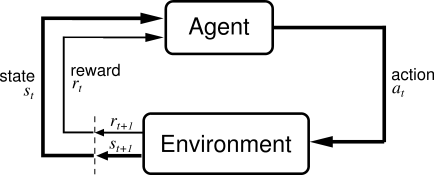
\includegraphics[keepaspectratio,width=\textwidth]{assets/agent_env}
\end{frame}

\begin{frame}{Notation}
  \begin{itemize}
    \item $x_t \in X$ (or $s_t$) are states, $u_t \in U$ (or $a_t$) are actions. 
    \item $r_t \in \mathbb{R}$ is a reward given by a \emph{reward function} $R : X \times U \rightarrow \mathbb{R}$.
    \item $P: X \times U \rightarrow X$ is a transition function.
    \item $\pi: X \rightarrow U$ is a \emph{policy} (or controller).
  \end{itemize}
\end{frame}

\begin{frame}{Value Functions}
  State value function\footfullcite{Sutton1998IntroductionTR}:
  \begin{equation}
    V_\pi(x) = \mathbb{E}\left[\sum_{t=0}^\top \gamma^t R(x_t, \pi(x_t)) \mid x_0 = x\right]
  \end{equation}
  satisfies Bellman equation
  \begin{equation}
    V_\pi(x) = \mathbb{E}\left[R(x, \pi(x)) + \gamma V_\pi(x_{t+1})\right]
  \end{equation}
\end{frame}

\begin{frame}{Policy Iteration}
  \begin{algorithm}[H]
      \DontPrintSemicolon
      \KwInput{An MDP $(X, U, R, P)$}
      \KwOutput{A policy $\pi$ optimizing rewards in the MDP}

      Initialize policy $\pi$ and $V_\pi$ \\
      \While {$\pi$ not stationary} {
        Estimate $V_\pi$ (\textbf{Policy Evaluation}) \\
        Set $\pi(x_t) = \argmax_{u_t} \left[r_t +  \gamma V_\pi(x_{t+1})\right]\ \forall x_t \in X$ \\ 
      }

      \textbf{Return} $\pi$

      \caption{Policy Iteration}
      \label{alg:stability_policy_iteration}
  \end{algorithm}
\end{frame}

\section{PARL in Three Parts}
\begin{frame}{Piecewise-Affine Reinforcement Learning}
  \scalebox{0.7} {
  \begin{algorithm}[H]
    \DontPrintSemicolon
    \SetAlgoLined
    \SetKwInOut{Input}{Input}
    \SetKwInOut{Output}{Output}
    \Input{A system to be controlled}
    \Output{A learned PARL controller}

    Sample reference points within state-space of $env$. \\
    Initialize $\hat{F}, \hat{V}$, and $\Pi$ to sensible defaults. \\
    \For{$i$ = $1\ldots training\_iterations$} {
      $data \leftarrow \emptyset$ \\
      \For{$j$ = $1\ldots num\_rollouts$} {
        $traj = do\_rollout(\Pi, env)$ \\
        $register\_experience(traj)$ \\
        $update\_dynamics(\hat{F})$ \\
        $update\_value\_function(\hat{V})$ \\
        $data \leftarrow data \cup traj$ \\
      }
      $update\_controller(\Pi, data)$ \\
      $data \leftarrow \emptyset$ \\
    }
    Return $\Pi$
    \caption{PARL}
  \end{algorithm}
  }
\end{frame}

\subsection{Partitioning}

\begin{frame}{What is a Partition?}
  We can loosely define a partition with indexing set $I$ of the state space $X$ as
  \begin{equation}
    P_I = \left\{\mathcal{V}_i \subseteq S\ \middle\vert 
      \begin{array}{l}
        i \in I, \\
        \bigcup_{i \in I}\mathcal{V}_i = S, \\
        \mathcal{V}_i \cap \mathcal{V}_j = \emptyset, \forall i \neq j
      \end{array}\right\}
  \end{equation}
\end{frame}

\begin{frame}{Implicit Voronoi Partition}
  Explicit polygonal partitions are expensive, so we define an implicit one by
  sampling \emph{reference points} and using a K-D Tree.\footfullcite{de1997computational}

  \begin{center}
    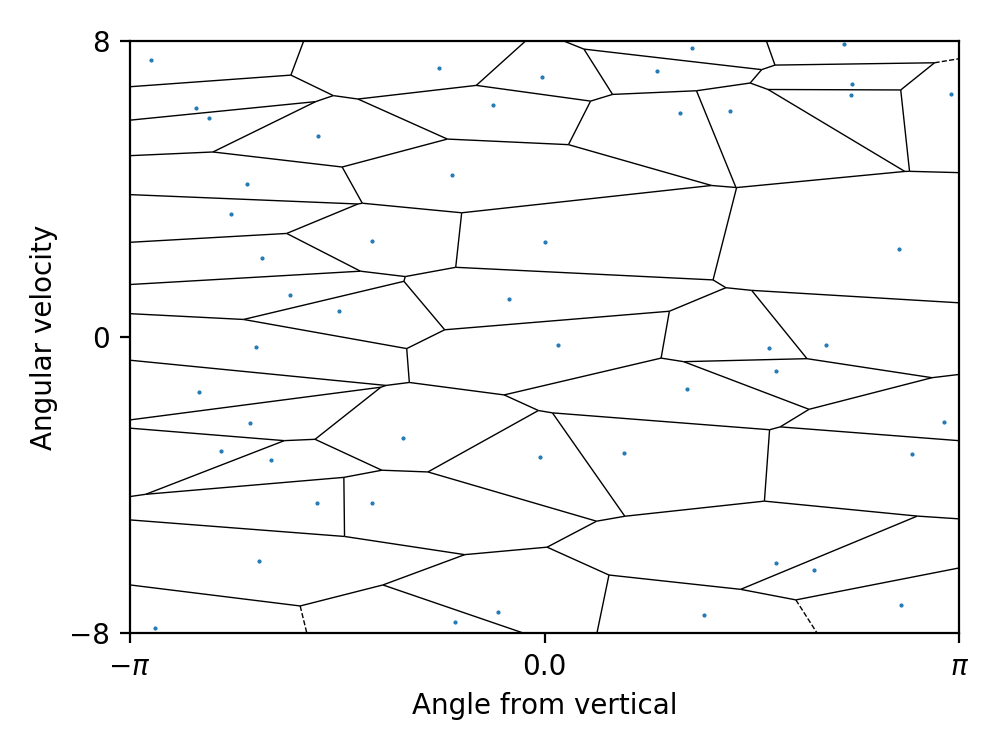
\includegraphics[keepaspectratio,width=0.8\textwidth]{assets/pendulum_voronoi}
  \end{center}
\end{frame}

\begin{frame}{Connections to Deep Neural Networks}
  Common deep neural network structures define implicit generalized Voronoi
  diagrams and piecewise-affine operators.\footfullcite{Balestriero2019TheGO} 

  \begin{center}
    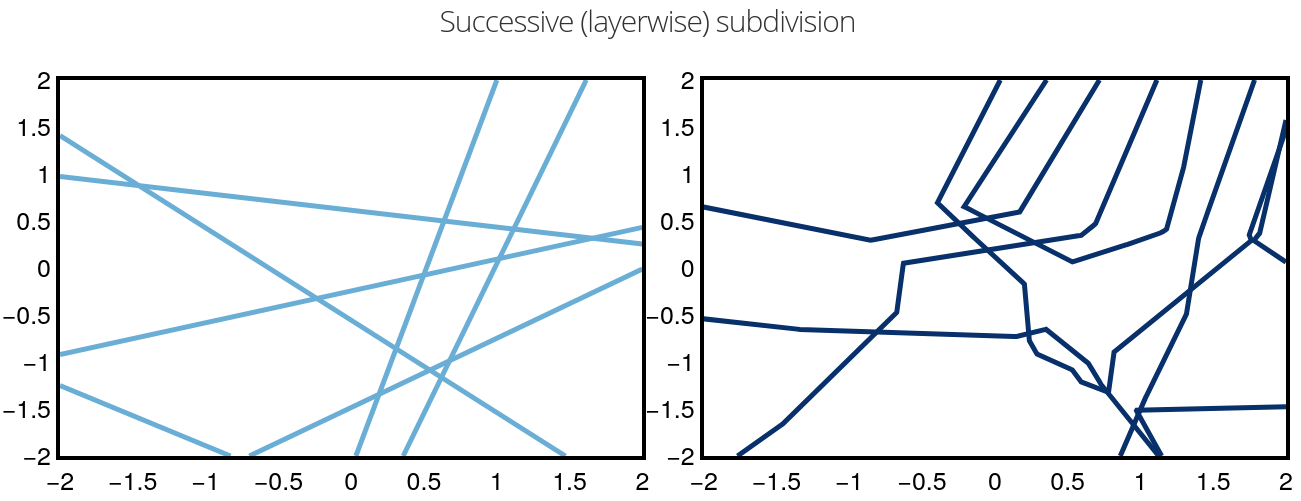
\includegraphics[keepaspectratio,width=0.8\textwidth]{assets/subdivision}
  \end{center}
\end{frame}

\subsection{Dynamics Estimation}

\begin{frame}{Local Linear Dynamics}
  We make a linear approximation to the local dynamics:
  \begin{equation}
    \hat{F}_{i}(\tilde{x}_t, u_t) = \hat{A}x_t + \hat{B}u_t + c 
  \end{equation}
  which can be estimated from data using \emph{Recursive Least Squares}
\end{frame}

\begin{frame}{Recursive Least Squares}
  The RLS filter is defined by
  \begin{align*}
    \phi_T &= \left[\begin{array}{l}x_t \\ u_t \end{array}\right] \\
    y_T &= x_{t+1}\\
    P_T &= P_{T-1} - \frac{P_{T-1}\phi_T \phi_T^\top P_{T-1}}{1 + \phi_T^\top P_{T-1} \phi_T} &\text{\emph{(Inverse sample covariance)}} \\
    \theta_T &= \theta_{T-1} + P_T \phi_T \left[y_T - \phi_T^\top \theta_{T-1} \right] &\text{\emph{(RLS parameter estimate)}}
  \end{align*}

  Note $\theta_T = \begin{bmatrix}\hat{A} \\ \hat{B}\end{bmatrix}$, and $\hat{c}$ can be estimated in a similar way.\footnote{See \url{http://cannontwo.com/assets/rls_notes.pdf}}
\end{frame}

\begin{frame}{Theoretical Guarantees}
  Assuming white noise corruption of the $y_T$ values, RLS converges almost
  surely to the true parameters. It can also be modified to deal with white
  noise corrupting $\phi_T$. However, $P_T$ must always have full rank.
\end{frame}

\begin{frame}{Practical Implementation}
  There are several implementation details:
  \begin{itemize}
    \item $P_0$ must be chosen arbitrarily
    \item Estimating $\hat{c}$ requires a little additional bookkeeping
    \item Forgetting factor $\lambda$ for time-varying parameters
  \end{itemize}
\end{frame}

\subsection{Value Function Approximation}

\begin{frame}{Local Value Function Approximation}
  Similar to the dynamics approximation, we make a linear approximation of the local dynamics:
  \begin{equation}
    \hat{V}^{\pi}_i(x_t) = V_0 + V_x^\top x_t
  \end{equation}
  which can be estimated using \emph{Least Squares Temporal Difference Learning}.
\end{frame}

\begin{frame}{Least Squares Temporal Difference Learning}
  The LSTD filter is a modified RLS filter, defined by:
  \begin{align*}
    \Delta &= \phi_T(x_t) - \gamma \phi_T(x_{t+1})\\
    C_{t+1} &= C_T - \frac{C_T \phi_T(x_t) \Delta^\top C_T}{1 + \Delta^\top C_t \phi_T(x_t)}\\
    d_{t+1} &= d_T + \phi_T(x_t)r_t
  \end{align*}
  and the corresponding parameters are given by $C_T d_T$, from which $V_0$ and $V_x$ can be extracted for each partition region.
\end{frame}

\begin{frame}{LSTD Theoretical Guarantees}
  LSTD has the same sort of theoretical results as the RLS filter, except that
  additional decorrelation conditions apply between $\Delta$ and $\phi_T(x_t)$.
\end{frame}

\begin{frame}{Practical Implementation}
  For PARL, we define
  \begin{align*}
    \phi_i(x_t) &= \begin{cases} \begin{bmatrix} x_t \\ 1 \end{bmatrix} & \text{for } x \in \mathcal{V}_i \\ 0  &\text{otherwise}\end{cases} \\
    \phi_T(x_t) &= \phi_i(x_t) \text{, stacked for all $i \in I$}
  \end{align*}
  This feature set defines a self-consistent piecewise-affine approximation to
  the value function on the PARL partition. However, it is computationally
  expensive to compute the LSTD approximation in this feature space. 
\end{frame}

\subsection{Controller Optimization}

\begin{frame}{Gradient-based Controller Updating}
  \fixme{TODO}
\end{frame}

\begin{frame}{Line Search on Dynamics and Value}
  \fixme{TODO}
\end{frame}

\begin{frame}{Theoretical Guarantees?}
  \fixme{TODO}
\end{frame}


\subsection{Results}

\begin{frame}{The Inverted Pendulum}
  \fixme{TODO}
\end{frame}

\begin{frame}{Reference Point Placement Experiments}
  \fixme{TODO}
\end{frame}

\begin{frame}{Interpretability Experiments}
  \fixme{TODO}
\end{frame}

\section{Stability of PARL Controllers}

\begin{frame}{Stability in Control}
  \fixme{TODO}
\end{frame}

\begin{frame}{Lyapunov Functions}
  \fixme{TODO}
\end{frame}

\begin{frame}{Kinds of Stability}
  \fixme{TODO}
\end{frame}

\begin{frame}{Piecewise-Affine Lyapunov Functions}
  \fixme{TODO}
\end{frame}

\begin{frame}{Mesh Refinement}
  \fixme{TODO}
\end{frame}

\begin{frame}{Inverted Pendulum Results}
  \fixme{TODO}
\end{frame}

\section{Future Work}

\begin{frame}{There's a lot}
  \fixme{TODO}
\end{frame}

\subsection{PARL+Planning}

\begin{frame}{Nominal Models}
  \fixme{TODO}
\end{frame}

\begin{frame}{Learning Errors}
  \fixme{TODO}
\end{frame}

\begin{frame}{Tracking Control and Model Updating}
  \fixme{TODO}
\end{frame}

\subsection{Theoretical Results}

\begin{frame}{PARL Algorithmic Stability}
  \fixme{TODO}
\end{frame}

\begin{frame}{PARL Algorithmic Robustness}
  \fixme{TODO}
\end{frame}

\subsection{Adaptive Partitioning}

\begin{frame}{Extension to Varying Mesh}
  \fixme{TODO}
\end{frame}

\begin{frame}{Adaptation Strategies}
  \fixme{TODO}
\end{frame}

\subsection{Explicit Uncertainty}

\begin{frame}{Sources of Uncertainty}
  \fixme{TODO}
\end{frame}

\begin{frame}{Integrating Uncertainty}
  \fixme{TODO}
\end{frame}

\begin{frame}{Priors?}
  \fixme{TODO}
\end{frame}

\section{Questions?}

\end{document}
